%%%%%%%%%%%%%%%%%%%%%%%%%%%%%%%%%%%%%%%%%%%%%%%%%%%%%%%%
\documentclass[10.5pt,a4paper]{article}% 文档格式
\usepackage{ctex,hyperref}% 输出汉字
% \usepackage{times}% 英文使用Times New Roman
%%%%%%%%%%%%%%%%%%%%%%%%%%%%%%%%%%%%%%%%%%%%%%%%%%%%%%%%
\title{\fontsize{22pt}{20pt}\selectfont% 小四字号,1.5倍行距
	{\heiti% 黑体 
		基于resnext101的手写汉字识别}}% 题目
%%%%%%%%%%%%%%%%%%%%%%%%%%%%%%%%%%%%%%%%%%%%%%%%%%%%%%%%
\author{\fontsize{12pt}{12pt}\selectfont% 小四字号,1.5倍行距
	{\fangsong% 仿宋
		李志远}\\% 标题栏脚注
	\fontsize{10.5pt}{15.75pt}\selectfont% 小五字号,1.5倍行距
	{\fangsong% 仿宋
		(南京农业大学 人工智能201)}}% 作者单位,“~”表示空格
%%%%%%%%%%%%%%%%%%%%%%%%%%%%%%%%%%%%%%%%%%%%%%%%%%%%%%%%
\date{}% 日期(这里避免生成日期)
%%%%%%%%%%%%%%%%%%%%%%%%%%%%%%%%%%%%%%%%%%%%%%%%%%%%%%%%
\usepackage{amsmath,amsfonts,amssymb}% 为公式输入创造条件的宏包
%%%%%%%%%%%%%%%%%%%%%%%%%%%%%%%%%%%%%%%%%%%%%%%%%%%%%%%%
\usepackage{graphicx}% 图片插入宏包
\usepackage{subfigure}% 并排子图
\usepackage{float}% 浮动环境,用于调整图片位置
\usepackage[export]{adjustbox}% 防止过宽的图片
%%%%%%%%%%%%%%%%%%%%%%%%%%%%%%%%%%%%%%%%%%%%%%%%%%%%%%%%
\usepackage{bibentry}
\usepackage{natbib}% 以上2个为参考文献宏包
%%%%%%%%%%%%%%%%%%%%%%%%%%%%%%%%%%%%%%%%%%%%%%%%%%%%%%%%
\usepackage{abstract}% 两栏文档,一栏摘要及关键字宏包
\renewcommand{\abstracttextfont}{\songti}% 摘要内容字体为宋体
%%%%%%%%%%%%%%%%%%%%%%%%%%%%%%%%%%%%%%%%%%%%%%%%%%%%%%%%
\usepackage{xcolor}% 字体颜色宏包
\newcommand{\red}[1]{\textcolor[rgb]{1.00,0.00,0.00}{#1}}
\newcommand{\blue}[1]{\textcolor[rgb]{0.00,0.00,1.00}{#1}}
\newcommand{\green}[1]{\textcolor[rgb]{0.00,1.00,0.00}{#1}}
\newcommand{\darkblue}[1]
{\textcolor[rgb]{0.00,0.00,0.50}{#1}}
\newcommand{\darkgreen}[1]
{\textcolor[rgb]{0.00,0.37,0.00}{#1}}
\newcommand{\darkred}[1]{\textcolor[rgb]{0.60,0.00,0.00}{#1}}
\newcommand{\brown}[1]{\textcolor[rgb]{0.50,0.30,0.00}{#1}}
\newcommand{\purple}[1]{\textcolor[rgb]{0.50,0.00,0.50}{#1}}% 为使用方便而编辑的新指令
%%%%%%%%%%%%%%%%%%%%%%%%%%%%%%%%%%%%%%%%%%%%%%%%%%%%%%%%
\usepackage{url}% 超链接
\usepackage{bm}% 加粗部分公式
\usepackage{multirow}
\usepackage{booktabs}
\usepackage{epstopdf}
\usepackage{epsfig}
\usepackage{longtable}% 长表格
\usepackage{supertabular}% 跨页表格
\usepackage{algorithm}
\usepackage{algorithmic}
\usepackage{changepage}% 换页
%%%%%%%%%%%%%%%%%%%%%%%%%%%%%%%%%%%%%%%%%%%%%%%%%%%%%%%%
\usepackage{tikz}
\tikzstyle{conv}=[rectangle, draw=black!80, fill=white!20, minimum size=2em]
\tikzstyle{add}=[rectangle, draw=black!80, fill=white!20, minimum size=2em]
\tikzstyle{group}=[rectangle, draw=black!80, fill=white!20, minimum size=2em]

%%%%%%%%%%%%%%%%%%%%%%%%%%%%%%%%%%%%%%%%%%%%%%%%%%%%%%%%
\usepackage{enumerate}% 短编号
\usepackage{caption}% 设置标题
\captionsetup[figure]{name=\fontsize{10pt}{15pt}\selectfont Figure}% 设置图片编号头
\captionsetup[table]{name=\fontsize{10pt}{15pt}\selectfont Table}% 设置表格编号头
%%%%%%%%%%%%%%%%%%%%%%%%%%%%%%%%%%%%%%%%%%%%%%%%%%%%%%%%
\usepackage{indentfirst}% 中文首行缩进
\usepackage[left=2.0cm,right=2.0cm,top=2.40cm,bottom=2.40cm]{geometry}% 页边距设置
\renewcommand{\baselinestretch}{1.5}% 定义行间距(1.5)
%%%%%%%%%%%%%%%%%%%%%%%%%%%%%%%%%%%%%%%%%%%%%%%%%%%%%%%%
\usepackage{fancyhdr} %设置全文页眉、页脚的格式
\pagestyle{fancy}
\hypersetup{colorlinks=true,linkcolor=black}% 去除引用红框,改变颜色

%%%%%%%%%%%%%%%%%%%%%%%%%%%%%%%%%%%%%%%%%%%%%%%%%%%%%%%%

\begin{document}% 以下为正文内容
	\maketitle% 产生标题,没有它无法显示标题
	%%%%%%%%%%%%%%%%%%%%%%%%%%%%%%%%%%%%%%%%%%%%%%%%%%%%%%%%
	\lhead{}% 页眉左边设为空
	\chead{}% 页眉中间设为空
	\rhead{}% 页眉右边设为空
	\lfoot{}% 页脚左边设为空
	\cfoot{\thepage}% 页脚中间显示页码
	\rfoot{}% 页脚右边设为空
	%%%%%%%%%%%%%%%%%%%%%%%%%%%%%%%%%%%%%%%%%%%%%%%%%%%%%%%%
	\begin{adjustwidth}{1.06cm}{1.06cm}
            \fontsize{9pt}{13.5pt}\heiti{摘要:}\songti 本文旨在探究在手写汉字识别任务中,使用不同的深度神经网络对性能的影响,并找到最优的网络结构。我在给定的数据集上进行了实验,并使用了常见的神经网络架构,包括ResNet101、ResNeXt101和ResNet152。我们使用9:1的训练集-测试集比率进行数据集划分,并在预处理时将所有样本resize为60*60大小的图片,并在训练时进行不大于30度的随机旋转。实验结果表明,使用ResNeXt101网络结构获得了最好的性能表现,准确率达到了99.2\%。在实验过程中,我们还尝试了使用数据增强、调整学习率等方法来优化模型性能,但结果表明这些方法并没有显著提高模型的准确率。综上所述,我们建议在手写汉字识别任务中使用ResNeXt101网络结构,以达到最佳性能。
	\end{adjustwidth}
	\begin{adjustwidth}{1.06cm}{1.06cm}
		\fontsize{9pt}{10pt}\selectfont{\heiti{关键词:}\songti{深度学习,残差神经网络,手写汉字识别}}\\
	\end{adjustwidth}

	\begin{adjustwidth}{1.06cm}{1.06cm}% 英文摘要内容
		\fontsize{9pt}{10pt}\selectfont{\heiti{\textbf{Abstract:}}\songti{This paper aims to explore the impact of using different deep neural networks on the performance of handwritten Chinese character recognition task, and find the optimal network structure. I performed experiments on the given dataset and used common neural network architectures including ResNet101, ResNeXt101, and ResNet152. We use a 9:1 training-test set ratio for dataset partitioning, and resize all samples to 60*60 sized images during preprocessing, and randomly rotate them by no more than 30 degrees during training. The experimental results show that the best performance is obtained by using the ResNeXt101 network structure, and the accuracy reaches 99.2\%. During the experiment, we also tried using data augmentation, adjusting the learning rate and other methods to optimize the model performance, but the results showed that these methods did not significantly improve the accuracy of the model. In summary, we propose to use the ResNeXt101 network structure in the handwritten Chinese character recognition task to achieve the best performance. }}
	\end{adjustwidth}
         \begin{adjustwidth}{1.06cm}{1.06cm}
		\fontsize{9pt}{10pt}\selectfont{\heiti{\textbf{Keywords:}}\songti{Deep Learning,Resnet,Chinese Handwriting Recognition}}\\
	\end{adjustwidth}
	\newpage% 从新的一页继续
        \section{整体思路}
        在手写汉字识别任务中,神经网络已经被证明是一种有效的工具。我的计划是使用ResNet101、ResNext101和ResNet152等不同的网络结构进行对比实验,并针对是否使用预训练模型进行了对比实验,以找到最佳性能的网络结构。\par
        实验的数据集已提前给出,图片偏小,因此不适合使用固定224大小输入的AlexNet,该数据集包含了500类汉字、每个汉字有80张图片。我将数据集划分了为训练集、测试集,以进行模型训练和评估。\par
        在训练神经网络时,我针对我的训练设备进行超参数的设置,例如学习率、批量大小、迭代次数等,以获得最佳性能。此外,考虑到汉字的绝对位置对其分类有较大影响,我仅使用了随机旋转进行数据增强,没有使用裁剪、翻转等手段,resnet等网络结构本身使用了batch normalization\cite{batchnorm}以防止过拟合,由于dropout\cite{dropout}与batch norm同时使用会影响性能,因此不另外设置dropout层。\par
        训练完成后,我对测试集进行了评估,并记录了各个网络结构的性能指标。由于分类数较大,混淆矩阵与roc曲线并不直观,因此此处没有使用。\par
        最后,我对实验结果进行了分析和总结,并提出改进方案。例如,你可以尝试其他的网络结构、优化算法或数据增强技巧,以进一步提高手写汉字识别的性能。
        \section{数据集}
        \subsection{数据集划分}
        我将整个数据集按照9:1的比率划分为训练集和测试集。训练集用于训练神经网络,测试集用于评估网络的性能。具体做法为将数据重新划分到train和test文件夹内,使用imagefolder类读取。
        \subsection{数据预处理}
        我将所有图像统一resize为了60x60像素的大小以使得所有图像具有相同的尺寸,方便输入到神经网络中进行训练和测试。同时,我使用了数据增强技术,在训练时进行不大于30度的随机旋转,可以使得神经网络更好地学习汉字的不同书写风格。
        \section{模型}
        \subsection{ResNet}
        ResNet(Residual Network)是一种深度卷积神经网络,它由何凯明等人于2015年提出\cite{He_2016_CVPR},并在ImageNet\cite{imagenet}图像识别和COCO\cite{coco}物体检测等任务中取得了非常好的结果。ResNet主要的创新点是引入了残差连接(residual connections)来解决深度神经网络训练时的梯度消失问题。\par
        \begin{figure}[H]
        \centering
            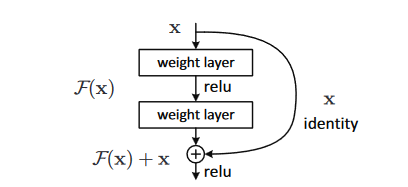
\includegraphics[width=0.48\textwidth]{residual block.png}
          \caption{Residual learning:a building block\cite{He_2016_CVPR}}
          \label{fig:resnet}
        \end{figure}
        传统的深度神经网络中,随着网络层数的增加,梯度会逐渐变得很小,导致无法正确地更新网络参数。为了解决这个问题,ResNet提出了残差学习的思想:即对于每个层,不再学习其直接映射,而是学习其残差映射,即输入与输出之间的差异。这样,网络就可以直接学习输入和输出之间的差异,而不必担心梯度消失的问题。\par
        在ResNet中,残差连接被添加到了卷积层中,以使得每个卷积层的输出不仅取决于该层的输入,还取决于该层之前所有层的输入。这种全局信息的融合可以帮助网络更好地学习特征,从而提高模型的准确率。ResNet中还使用了批量归一化和池化层等技术,以进一步提高网络的性能。\par
        ResNet的网络结构非常深,可以达到1000多层,但其计算量并不比传统的浅层网络大。这使得ResNet成为了处理大规模图像数据的首选网络之一。同时,ResNet的成功也启示了后续研究者提出了更加深入的残差网络,如ResNeXt、Wide ResNet\cite{wideresnet}等。
        \subsection{ResNext}
        ResNeXt(Residual Next)是一种基于ResNet的残差网络结构,由微软亚洲研究院的Xie Saining等人于2016年提出\cite{xie2017aggregated}。ResNeXt主要的创新点是使用了组卷积(group convolution)来进一步提升网络的性能和可扩展性。\par
        \begin{figure}[H]
        \centering
            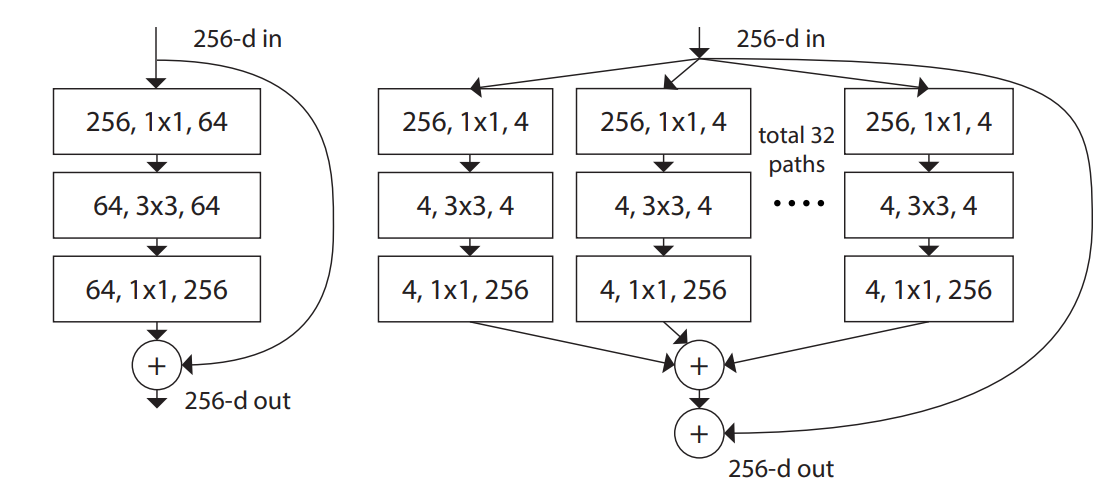
\includegraphics[width=0.8\textwidth]{resnext.png}
          \caption{\textbf{Right}: A block of ResNeXt with cardinality = 32, with roughly the same complexity. A layer is shown as (\# in channels, filter size, \# out channels)\cite{xie2017aggregated}}
          \label{fig:resnext_resnet}
        \end{figure}
        组卷积是一种卷积操作,将输入的特征图分成若干个组,每个组之间进行卷积,最后将各组的卷积结果拼接在一起。在ResNeXt中,组卷积被广泛应用于卷积层,可以有效减少参数数量和计算量,并提高了模型的准确率。组卷积的思想类似于Inception模块中的分支结构,但ResNeXt中的组卷积更加灵活,可以根据具体任务的需求进行组合。\par
        ResNeXt的结构与ResNet类似,但在卷积层中引入了组卷积,使得网络可以更好地学习特征。ResNeXt还采用了批量归一化和池化层等技术来进一步提高网络的性能。与ResNet相比,ResNeXt的计算量和参数数量都要小,但准确率却有显著的提升。\par
        ResNeXt的成功启示了后续研究者对残差网络的深入探索,如DenseNet\cite{densenet}等。同时,ResNeXt也被广泛应用于图像分类、目标检测和语义分割等领域,并在多项比赛中取得了优异的成绩。
        \section{实验}
        \subsection{超参数}
        我针对每个网络都至少训练了40个周期,学习率设置为1e-3,权重衰退值设置为1e-4,批量大小为64,momentum为0.9,其中resnet101训练时间约为2min/epoch,resnext101$\_ 32 \times 4d$ 约为 4min/epoch。\par
        \subsection{网络比较}
        我使用了resnet101、resnext101\_32$\times$ 4d、resnet152网络结构,使用SGD、Adam优化器进行训练并将结果进行了对比,并针对是否使用预训练参数进行了对比实验,最终选择了最优的结果作为本次课设的模型。
        \subsection{resnet101表现}
        \subsubsection{模型结果}
            首先下图为resnet101的最优结果的训练过程中训练、验证的损失与准确率。resnet101的预训练模型在实验条件下验证集的准确率可达93.3\%。\par
            \begin{figure}[H]
            \centering
                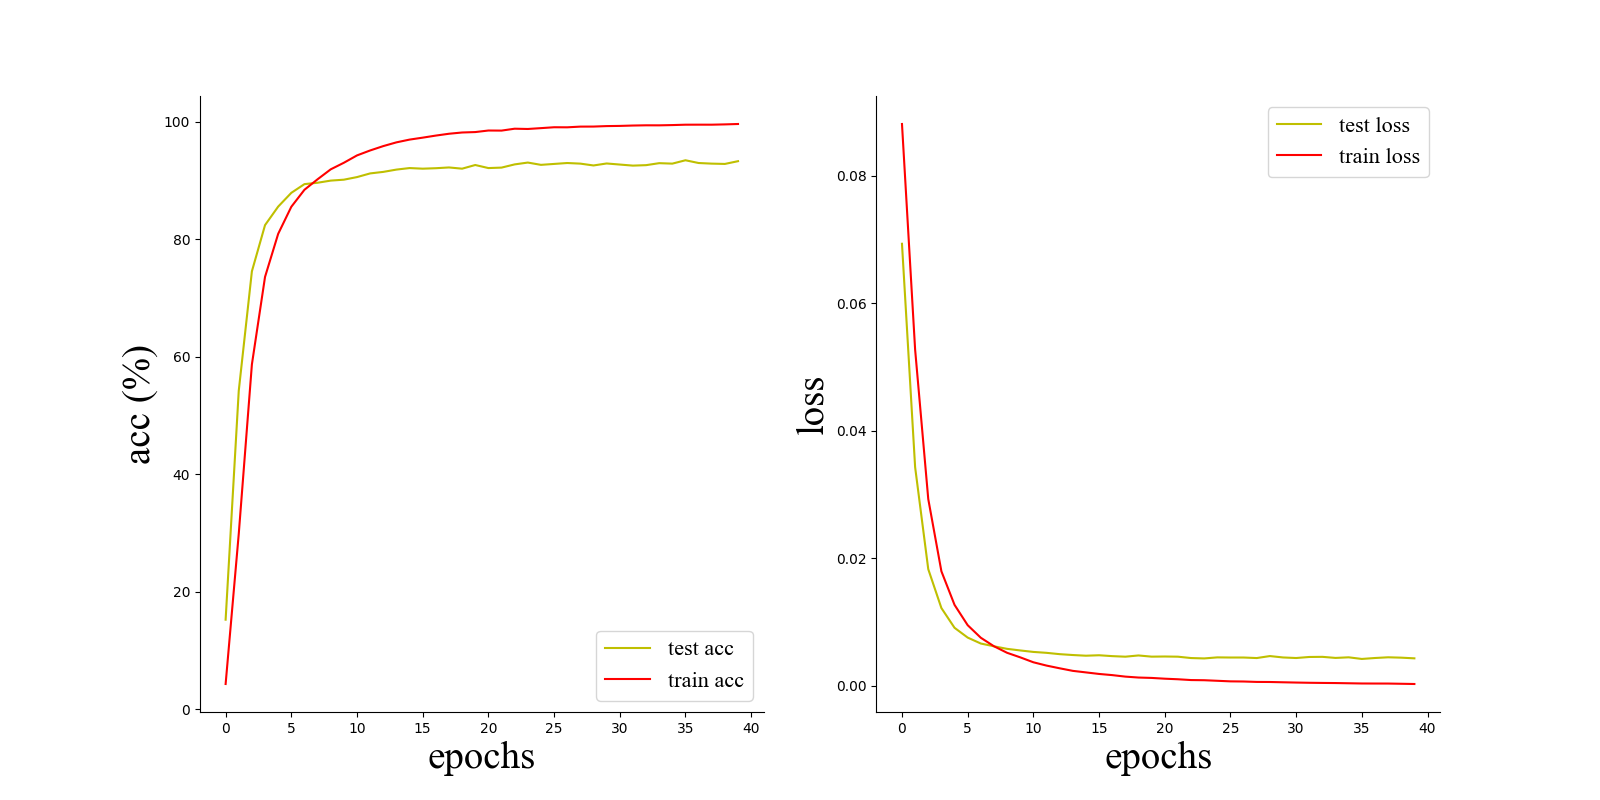
\includegraphics[width=0.8\textwidth]{resnet101_pretrained.png}
              \caption{resnet101\_pretrained训练过程及结果}
              \label{fig:resnet101_best_result}
            \end{figure}
        \subsubsection{预训练模型对比实验}
            我们在SGD、resnet101条件下设置了是否使用预训练模型进行训练进行对比,结果如下:
            \begin{figure}[H]% 插入两张图片并且并排
            	\centering
            	\begin{minipage}{0.48\textwidth}
            		\centering
            		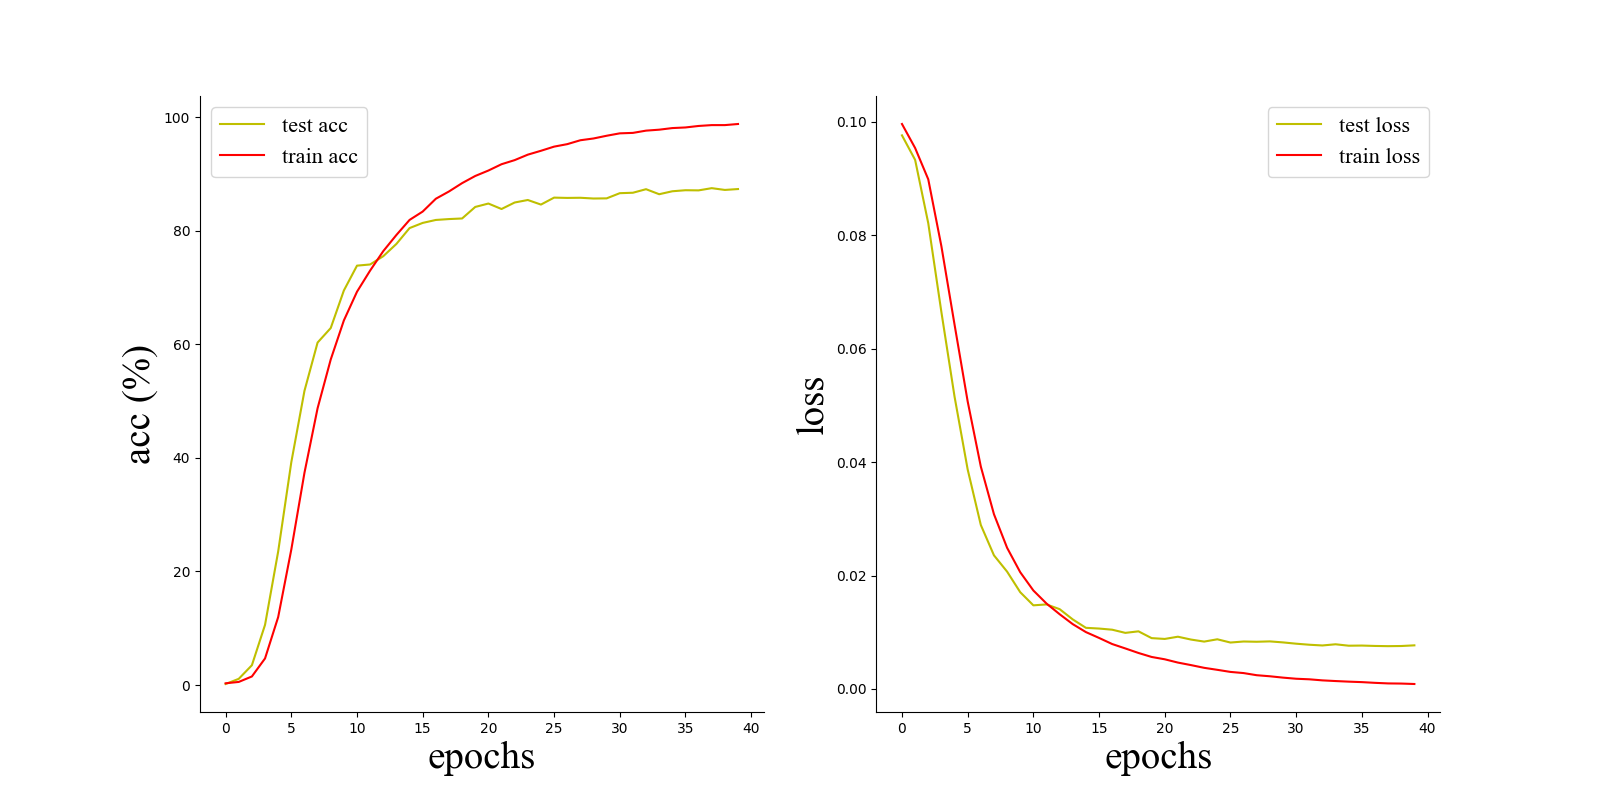
\includegraphics[width=\textwidth]{resnet101.png}
            		\caption{不使用预训练模型}
            	\end{minipage}
            	\hspace{0cm}% 图片间距
            	\hfill% 撑满整行
            	\begin{minipage}{0.48\textwidth}
            		\centering
            		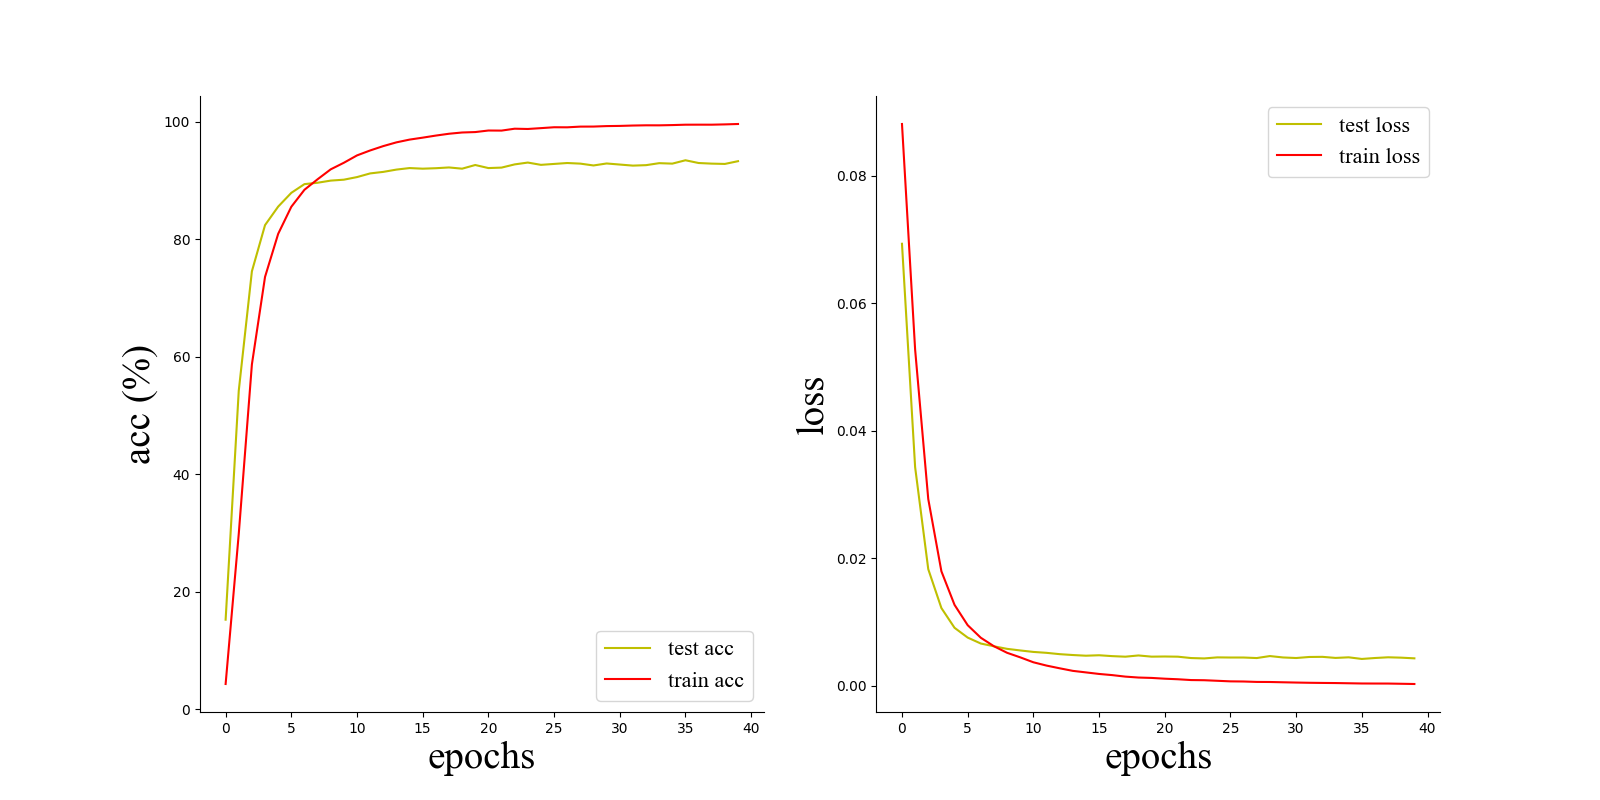
\includegraphics[width=\textwidth]{resnet101_pretrained.png}
            		\caption{使用预训练模型}
            	\end{minipage}
            \end{figure}
            明显可以看出使用预训练模型后模型泛化能力更强、更快收敛。下表为数据对比
            \begin{table}[!ht]
            \centering
            \begin{tabular}{|l|l|l|}
            \hline
                模型 & 最高准确率 & 到达80\%所需epochs \\ \hline
                resnet101 & 87.5\% & 15 \\ \hline
                resnet101\_pretrained & 93.46\% & 4 \\ \hline
            \end{tabular}
            \caption{是否使用预训练模型进行的数据对比}
            \end{table}
        \subsubsection{优化器对比实验}
            我们在使用预训练模型的resnet101设置分别使用SGD与Adam优化器进行训练,并将结果进行对比:
            \begin{figure}[H]% 插入两张图片并且并排
            	\centering
            	\begin{minipage}{0.48\textwidth}
            		\centering
            		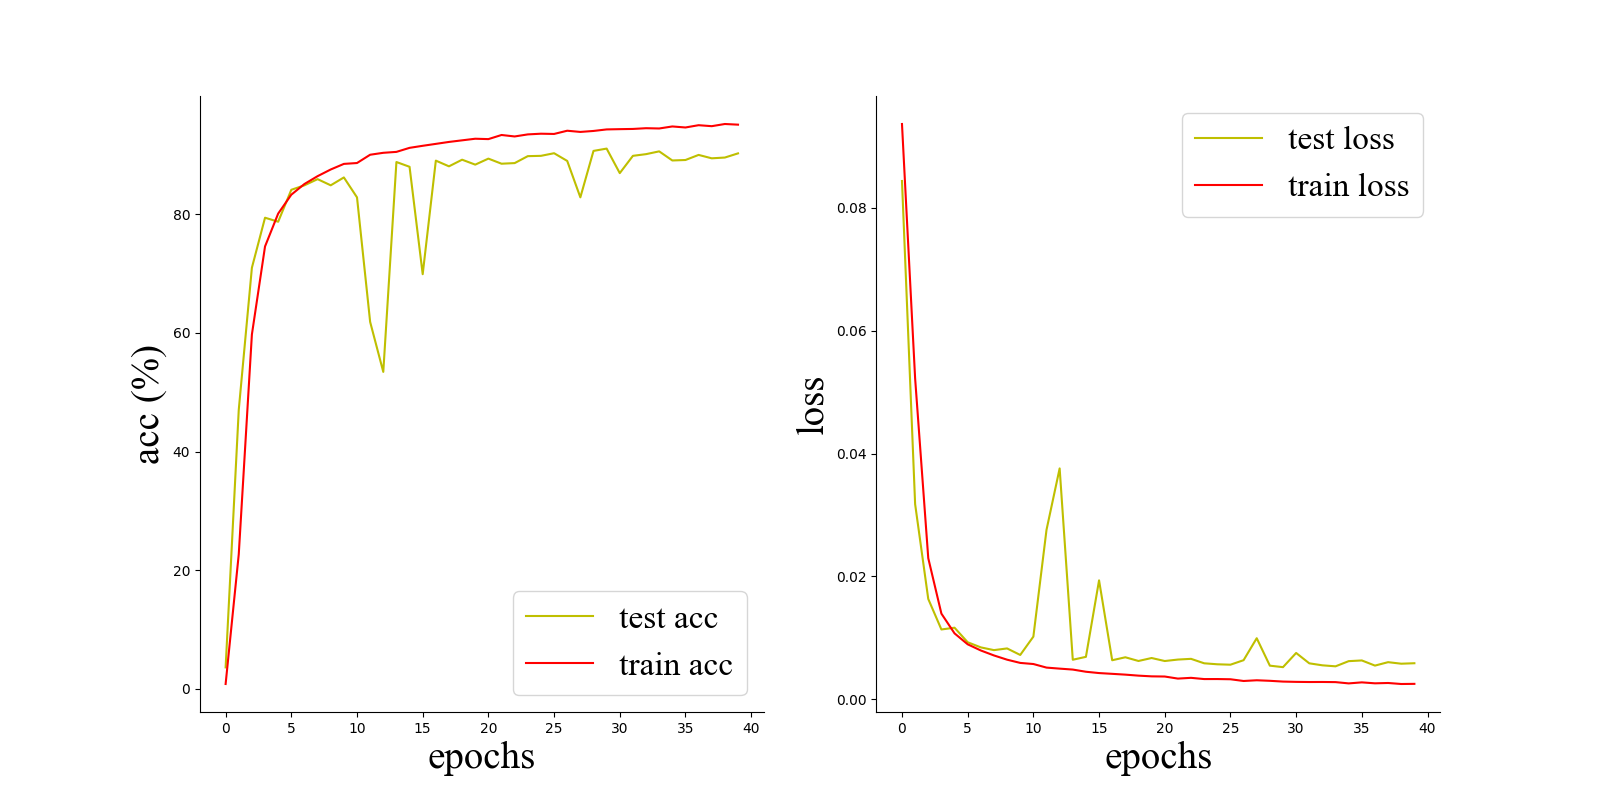
\includegraphics[width=\textwidth]{resnet101_pretrained_adam.png}
            		\caption{Adam}
            	\end{minipage}
            	\hspace{0cm}% 图片间距
            	\hfill% 撑满整行
            	\begin{minipage}{0.48\textwidth}
            		\centering
            		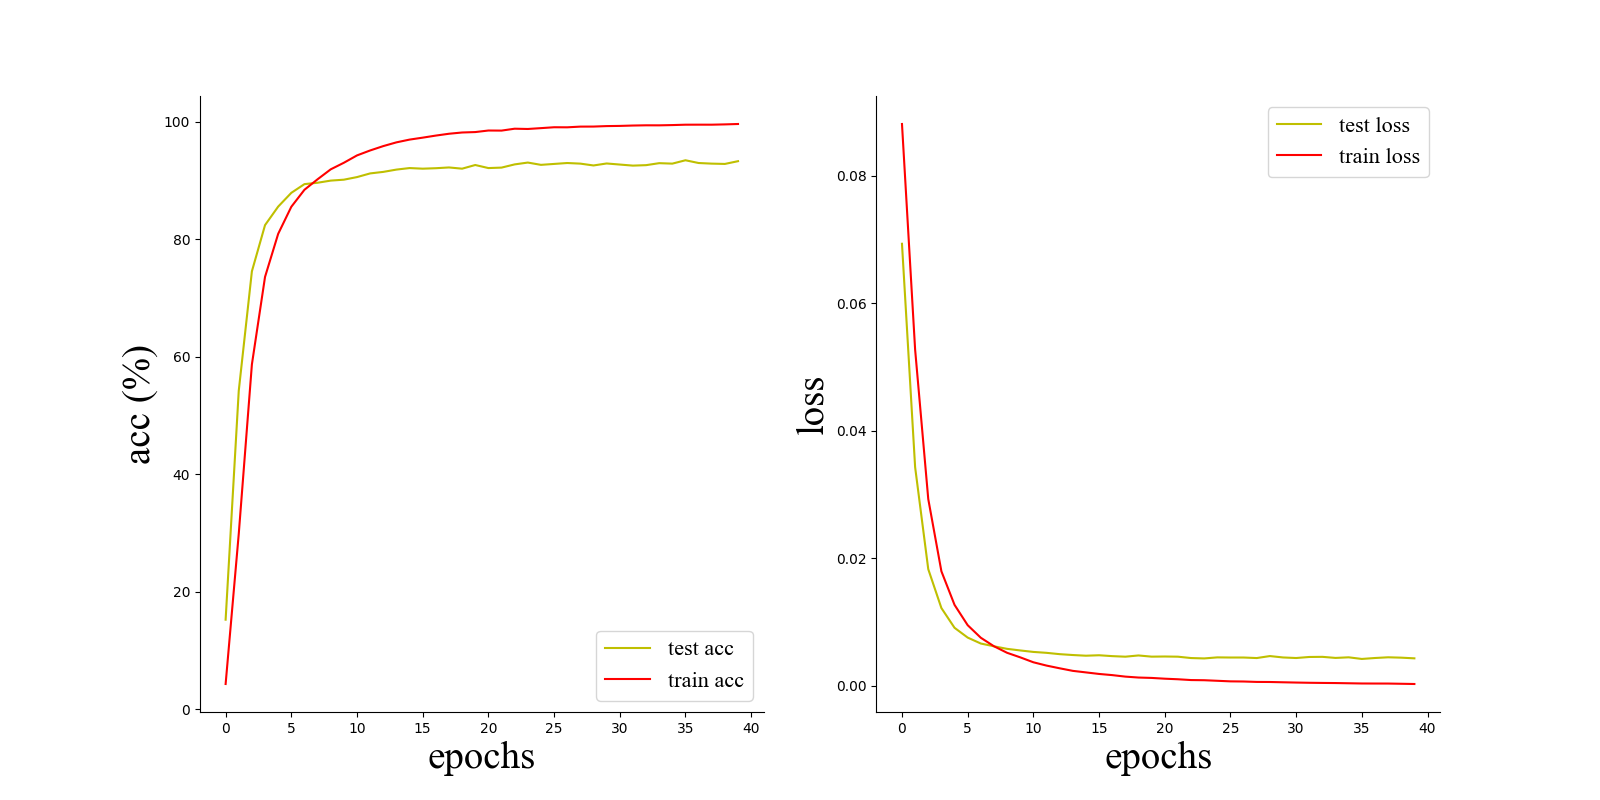
\includegraphics[width=\textwidth]{resnet101_pretrained.png}
            		\caption{SGD}
            	\end{minipage}
            \end{figure}
            综合来看,在选择恰当的学习率后,SGD的表现要优于Adam,同时SGD的训练过程也更加稳定;Adam的优势在于它对学习率不是很敏感,调参方面会比较方便。实验中SGD最高准确率为93.46\%,Adam为91.12\%。\par
            因此在后续两个网络的训练中,我们均使用预训练模型与SGD,其它组合我也实验过,为避免重复介绍这里只展示最好结果。
        \subsection{resnet152表现}
        resnet152的预训练模型在SGD条件下验证集的准确率可达93.28\%,下图为其训练过程中训练集、验证集的损失和准确率。
        \begin{figure}[H]
            \centering
                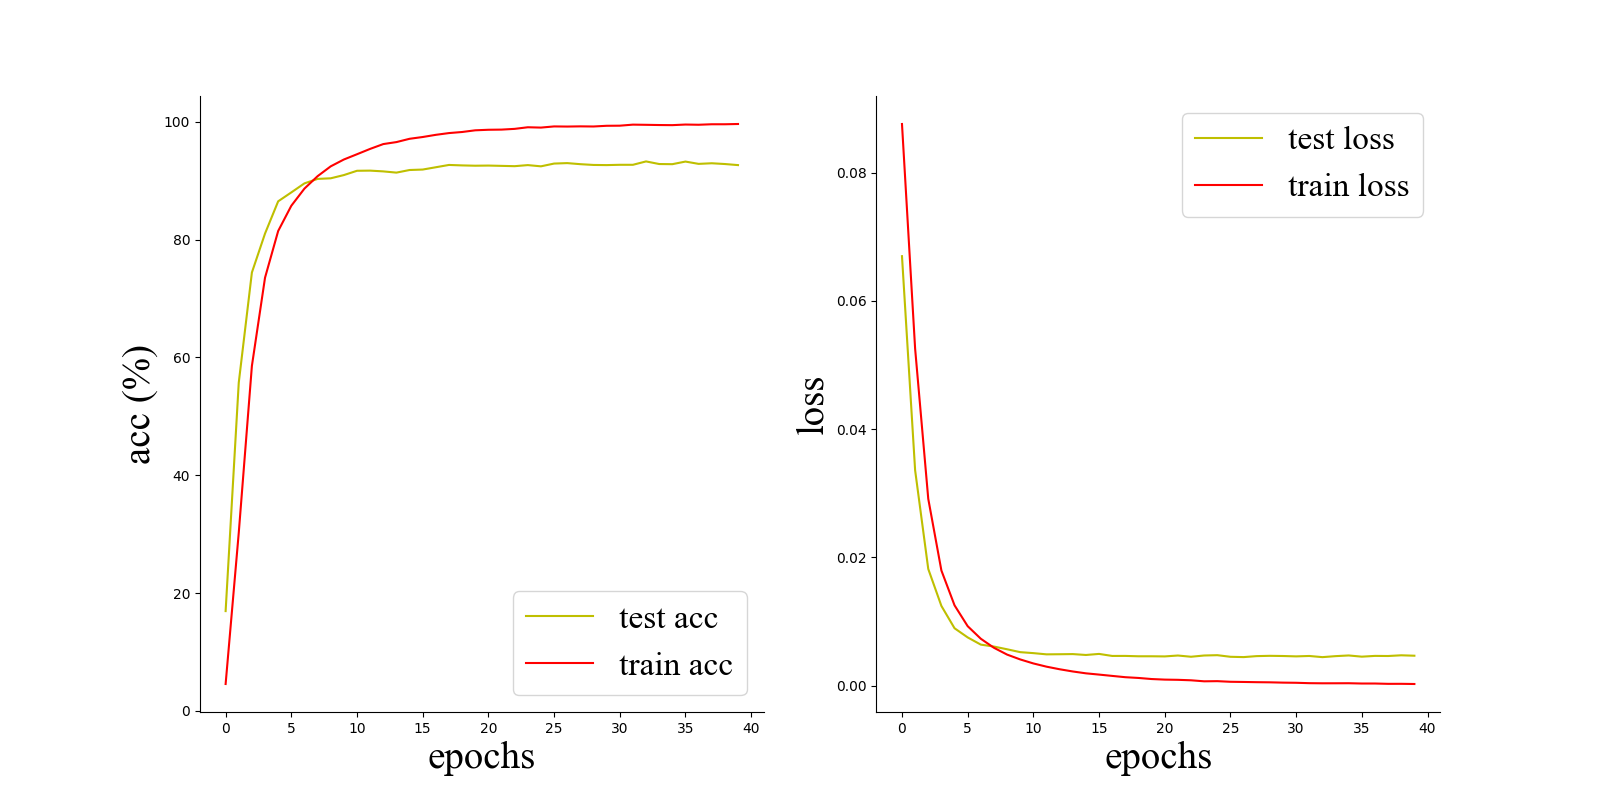
\includegraphics[width=0.8\textwidth]{resnet152_pretrained.png}
              \caption{resnet152\_pretrained训练过程及结果}
              \label{fig:resnet152_best_result}
        \end{figure}
        \subsection{resnext101\_32$\times$4d表现}
        resnext101的预训练模型在SGD条件下验证集的准确率可达94.01\%,下图为其训练过程中训练集、验证集的损失和准确率。
        \begin{figure}[H]
            \centering
                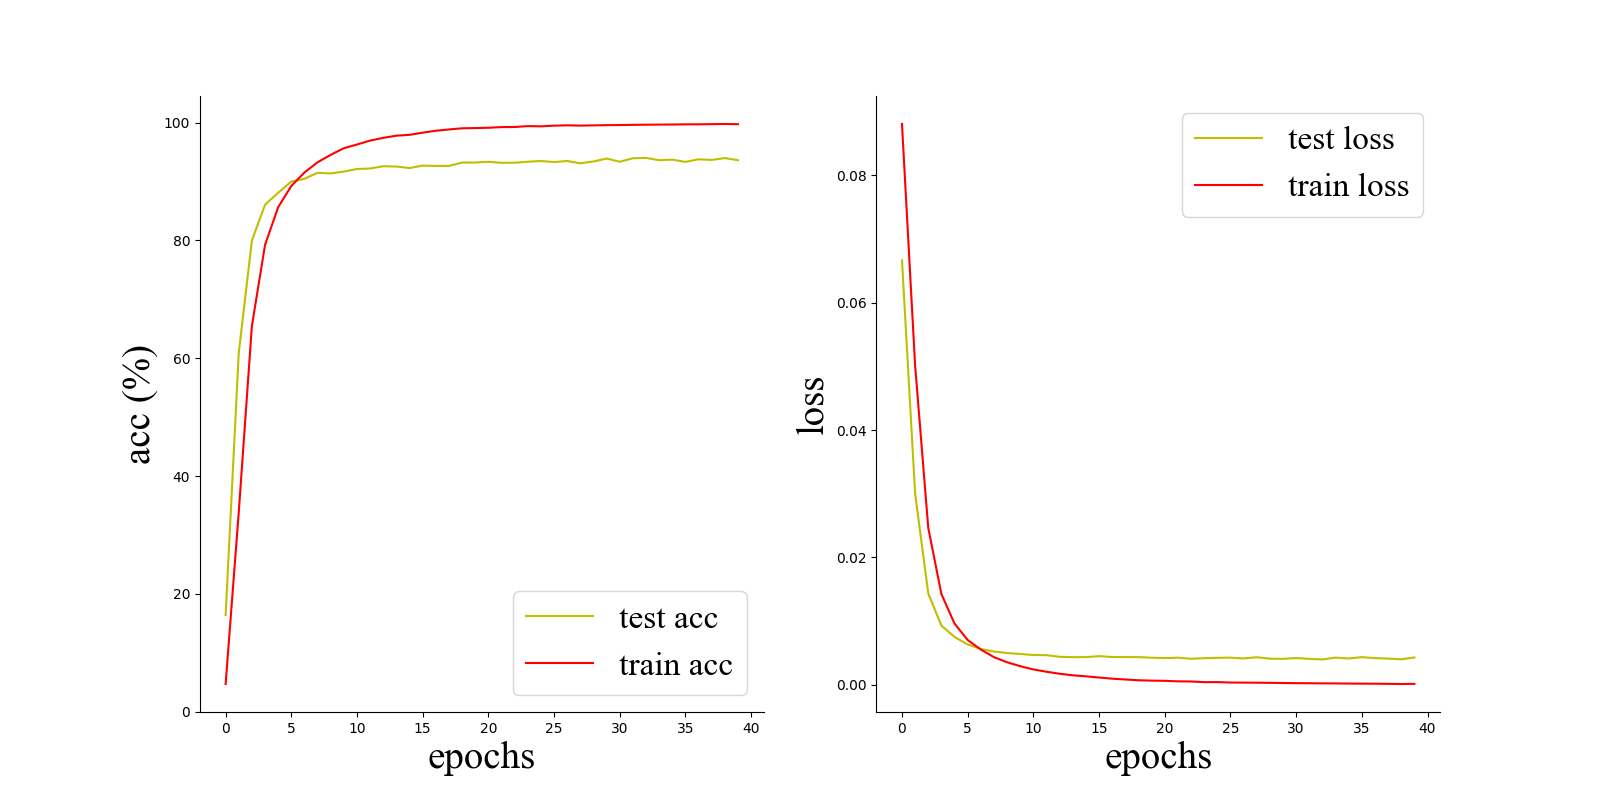
\includegraphics[width=0.8\textwidth]{resnext101_pretrained.png}
              \caption{resnext101\_pretrained训练过程及结果}
              \label{fig:resnext101_best_result}
        \end{figure}
        \subsection{结果}
        综上所述,我选择resnext101\_32$\times$8d作为本次课设的模型,其在实验条件下验证集的准确率最高,为94.01\%。其实验条件设置如下:\par
        \begin{table}[!ht]
        \centering
        \begin{tabular}{|l|l|}
        \hline
            超参数 & 值 \\ \hline
            learning rate & 1e-3 \\ \hline
            weight decay & 1e-4 \\ \hline
            momentum & 0.9 \\ \hline
            batch size & 64 \\ \hline
             epochs & 40 \\ \hline
        \end{tabular}
        \caption{超参数设置}
         \end{table}
        
        \section{结语}
        在这次的手写汉字识别的神经网络设计报告中,我使用了多种不同的网络结构进行对比实验,并最终确定了最优性能的网络结构。通过这个过程,我深入了解了神经网络在图像分类领域的应用,掌握了如何选择神经网络模型以及优化器、调参使得模型性能变高。\par
        在实验过程中,我也遇到了各种问题和挑战,但是通过不断尝试和调整,最终达到了预期的结果。这个过程让我更加深入地理解了神经网络的运作机制和优化方法,并增强了我解决实际问题的能力和信心。\par
        尤其重要的一点是,我又学到了很多模型展示的技巧,或者说将模型结果展示在论文/报告当中的方式,这是我之前没有考虑到的。总的说来,这次的课程设计让我受益匪浅,提高了我的专业技能和学术素养。我相信这些经验和知识将在未来的学习和工作中发挥重要作用。
\newpage
\bibliographystyle{plain}
\bibliography{my}

\end{document}% 结束文档编辑,后面写啥都编译不出来
